
\section{Assembling the Power Board}
The power board is at the heart of the electronics kit and for this reason should be assembled first. You will need a copy of the \textbf{Power Board Outline} for this section.

\subsection{Switches}
\begin{enumerate}
\item Connect the \textbf{Charge/Run Switch} to the Power Board. 
\item Connect the \textbf{On/Off Switch} to the Power Board - be careful to locate the correct socket. Leave the switch in the `Off' position.
\end{enumerate}

\subsection{Power USB Hub}
\begin{enumerate}
\item Use the \textbf{USB Hub Power Connector} to connect the Hub to the Power Board
\item Use the \textbf{USB Cable} to connect the Hub to the `Disk 2' USB socket on the Slug - see Figure \ref{fig:slug-side}
\item Insert both \textbf{USB Keys} into sockets on the USB Hub
\end{enumerate}

\begin{figure}[h!]
\center
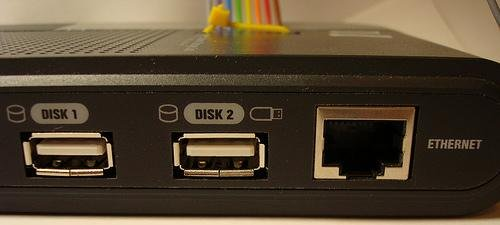
\includegraphics[scale=0.6]{slug-side-view}
\caption{Side view of the Slug's USB Ports}
\label{fig:slug-side}
\end{figure}


\subsection{The Slug}
Identify the Slug's Pin Header on the Power Board and \textbf{carefully} plug the Slug's multicoloured ribbon cable into it. Be sure to orientate the socket correctly, before applying force. This cable provides both power and data connections between the slug and, indirectly, all the SR modules.

\subsection{The Webcam}
Plug the \textbf{USB Webcam} into one of the spare USB sockets on the USB Hub.

\subsection{Fuse}
Your Power Board should have been supplied with a fuse already fitted. If yours hasn't, then contact a SR member as soon as possible.

\subsection{Battery \& Charger}
Connect the {\bf battery} to the {\bf Battery Connector} and plug the other end into the correct socket on the Power Board. {\bf Check the polarity carefully!}

Initially the battery will be uncharged, so plug the {\bf Battery Charger} into the socket on the Power Board and turn it on at the mains.


\subsection{Stop}
At this point you have assembled the minimum amount of kit to power up your robot. Ensure the Charge/Run Switch is in charge mode (see Power Board Documentation) and put the On/Off switch into the On position. If you have made no mistakes so far, the LEDs on the Power Board will be lit, the Slug will be flashing, and the lights on the USB hub and keys will also flash.

You may, at this point, write some python code to control the Power Board LEDs to satisfy yourself that everything is working.

